\documentclass[journal,12pt,twocolumn]{IEEEtran}
\usepackage{setspace}
\usepackage{gensymb}
\usepackage{caption}
%\usepackage{multirow}
%\usepackage{multicolumn}
%\usepackage{subcaption}
%\doublespacing
\singlespacing
\usepackage{csvsimple}
\usepackage{amsmath}
\usepackage{multicol}
%\usepackage{enumerate}
\usepackage{amssymb}
%\usepackage{graphicx}
\usepackage{newfloat}
%\usepackage{syntax}
\usepackage{listings}
\usepackage{color}
\usepackage{tikz}
\usepackage{graphicx}
\usetikzlibrary{shapes,arrows}

%\usepackage{graphicx}
%\usepackage{amssymb}
%\usepackage{relsize}
%\usepackage[cmex10]{amsmath}
%\usepackage{mathtools}
%\usepackage{amsthm}
%\interdisplaylinepenalty=2500
%\savesymbol{iint}
%\usepackage{txfonts}
%\restoresymbol{TXF}{iint}
%\usepackage{wasysym}
\usepackage{amsthm}
\usepackage{mathrsfs}
\usepackage{txfonts}
\usepackage{stfloats}
\usepackage{cite}
\usepackage{cases}
\usepackage{mathtools}
\usepackage{caption}
\usepackage{enumerate}	
\usepackage{enumitem}
\usepackage{amsmath}
%\usepackage{xtab}
\usepackage{longtable}
\usepackage{multirow}
%\usepackage{algorithm}
%\usepackage{algpseudocode}
\usepackage{enumitem}
\usepackage{mathtools}
\usepackage{hyperref}
%\usepackage[framemethod=tikz]{mdframed}
\usepackage{listings}
    %\usepackage[latin1]{inputenc}                                 %%
    \usepackage{color}                                            %%
    \usepackage{array}                                            %%
    \usepackage{longtable}                                        %%
    \usepackage{calc}                                             %%
    \usepackage{multirow}                                         %%
    \usepackage{hhline}                                           %%
    \usepackage{ifthen}                                           %%
  %optionally (for landscape tables embedded in another document): %%
    \usepackage{lscape}     


\usepackage{url}
\def\UrlBreaks{\do\/\do-}


%\usepackage{stmaryrd}


%\usepackage{wasysym}
%\newcounter{MYtempeqncnt}
\DeclareMathOperator*{\Res}{Res}
%\renewcommand{\baselinestretch}{2}
\renewcommand\thesection{\arabic{section}}
\renewcommand\thesubsection{\thesection.\arabic{subsection}}
\renewcommand\thesubsubsection{\thesubsection.\arabic{subsubsection}}

\renewcommand\thesectiondis{\arabic{section}}
\renewcommand\thesubsectiondis{\thesectiondis.\arabic{subsection}}
\renewcommand\thesubsubsectiondis{\thesubsectiondis.\arabic{subsubsection}}

% correct bad hyphenation here
\hyphenation{op-tical net-works semi-conduc-tor}

%\lstset{
%language=C,
%frame=single, 
%breaklines=true
%}

%\lstset{
	%%basicstyle=\small\ttfamily\bfseries,
	%%numberstyle=\small\ttfamily,
	%language=Octave,
	%backgroundcolor=\color{white},
	%%frame=single,
	%%keywordstyle=\bfseries,
	%%breaklines=true,
	%%showstringspaces=false,
	%%xleftmargin=-10mm,
	%%aboveskip=-1mm,
	%%belowskip=0mm
%}

%\surroundwithmdframed[width=\columnwidth]{lstlisting}
\def\inputGnumericTable{}                                 %%
\lstset{
%language=C,
frame=single, 
breaklines=true,
columns=fullflexible
}

\begin{document}
%
\tikzstyle{block} = [rectangle, draw,
    text width=3em, text centered, minimum height=3em]
\tikzstyle{sum} = [draw, circle, node distance=3cm]
\tikzstyle{input} = [coordinate]
\tikzstyle{output} = [coordinate]
\tikzstyle{pinstyle} = [pin edge={to-,thin,black}]

\theoremstyle{definition}
\newtheorem{theorem}{Theorem}[section]
\newtheorem{problem}{Problem}
\newtheorem{proposition}{Proposition}[section]
\newtheorem{lemma}{Lemma}[section]
\newtheorem{corollary}[theorem]{Corollary}
\newtheorem{example}{Example}[section]
\newtheorem{definition}{Definition}[section]
%\newtheorem{algorithm}{Algorithm}[section]
%\newtheorem{cor}{Corollary}
\newcommand{\BEQA}{\begin{eqnarray}}
\newcommand{\EEQA}{\end{eqnarray}}
\newcommand{\define}{\stackrel{\triangle}{=}}

\bibliographystyle{IEEEtran}
%\bibliographystyle{ieeetr}

\providecommand{\nCr}[2]{\,^{#1}C_{#2}} % nCr
\providecommand{\nPr}[2]{\,^{#1}P_{#2}} % nPr
\providecommand{\mbf}{\mathbf}
\providecommand{\pr}[1]{\ensuremath{\Pr\left(#1\right)}}
\providecommand{\qfunc}[1]{\ensuremath{Q\left(#1\right)}}
\providecommand{\sbrak}[1]{\ensuremath{{}\left[#1\right]}}
\providecommand{\lsbrak}[1]{\ensuremath{{}\left[#1\right.}}
\providecommand{\rsbrak}[1]{\ensuremath{{}\left.#1\right]}}
\providecommand{\brak}[1]{\ensuremath{\left(#1\right)}}
\providecommand{\lbrak}[1]{\ensuremath{\left(#1\right.}}
\providecommand{\rbrak}[1]{\ensuremath{\left.#1\right)}}
\providecommand{\cbrak}[1]{\ensuremath{\left\{#1\right\}}}
\providecommand{\lcbrak}[1]{\ensuremath{\left\{#1\right.}}
\providecommand{\rcbrak}[1]{\ensuremath{\left.#1\right\}}}
\theoremstyle{remark}
\newtheorem{rem}{Remark}
\newcommand{\sgn}{\mathop{\mathrm{sgn}}}
\providecommand{\abs}[1]{\left\vert#1\right\vert}
\providecommand{\res}[1]{\Res\displaylimits_{#1}} 
\providecommand{\norm}[1]{\left\Vert#1\right\Vert}
\providecommand{\mtx}[1]{\mathbf{#1}}
\providecommand{\mean}[1]{E\left[ #1 \right]}
\providecommand{\fourier}{\overset{\mathcal{F}}{ \rightleftharpoons}}
%\providecommand{\hilbert}{\overset{\mathcal{H}}{ \rightleftharpoons}}
\providecommand{\system}{\overset{\mathcal{H}}{ \longleftrightarrow}}
	%\newcommand{\solution}[2]{\textbf{Solution:}{#1}}
\newcommand{\solution}{\noindent \textbf{Solution: }}
\newcommand{\myvec}[1]{\ensuremath{\begin{pmatrix}#1\end{pmatrix}}}
\providecommand{\dec}[2]{\ensuremath{\overset{#1}{\underset{#2}{\gtrless}}}}
\DeclarePairedDelimiter{\ceil}{\lceil}{\rceil}
%\numberwithin{equation}{section}
%\numberwithin{problem}{subsection}
%\numberwithin{definition}{subsection}
\makeatletter
\@addtoreset{figure}{section}
\makeatother

\let\StandardTheFigure\thefigure
%\renewcommand{\thefigure}{\theproblem.\arabic{figure}}
\renewcommand{\thefigure}{\thesection}


%\numberwithin{figure}{subsection}

%\numberwithin{equation}{subsection}
%\numberwithin{equation}{section}
%\numberwithin{equation}{problem}
%\numberwithin{problem}{subsection}
\numberwithin{problem}{section}
%%\numberwithin{definition}{subsection}
%\makeatletter
%\@addtoreset{figure}{problem}
%\makeatother
\makeatletter
\@addtoreset{table}{section}
\makeatother

\let\StandardTheFigure\thefigure
\let\StandardTheTable\thetable
\let\vec\mathbf
\numberwithin{equation}{section}

\vspace{3cm}


\title{%Convex Optimization in Python
	Random Numbers
}
%\title{
%	\logo{Matrix Analysis through Octave}{\begin{center}\includegraphics[scale=.24]{tlc}\end{center}}{}{HAMDSP}
%}

% paper title
% can use linebreaks \\ within to get better formatting as desired
%\title{Matrix Analysis through Octave}
%
%
% author names and IEEE memberships
% note positions of commas and nonbreaking spaces ( ~ ) LaTeX will not break
% a structure at a ~ so this keeps an author's name from being broken across
% two lines.
% use \thanks{} to gain access to the first footnote area
% a separate \thanks must be used for each paragraph as LaTeX2e's \thanks
% was not built to handle multiple paragraphs
%

\author{D. Chandrahas\\AI21BTECH11010}
\maketitle

\tableofcontents

\bigskip

\renewcommand{\thefigure}{\theenumi}
\renewcommand{\thetable}{\theenumi}

\begin{abstract}
This manual provides a simple introduction to the generation of random numbers
\end{abstract}
%%
\section{Uniform Random Numbers}
Let $U$ be a uniform random variable between 0 and 1.
\begin{enumerate}[label=\thesection.\arabic*
,ref=\thesection.\theenumi]
\item Generate $10^6$ samples of $U$ using a C program and save into a file called uni.dat .

\solution Compile and execute the following C program
\begin{lstlisting}
codes/exrand.c
codes/coeffs.h
\end{lstlisting}

\item
Load the uni.dat file into python and plot the empirical CDF of $U$ using the samples in uni.dat. The CDF is defined as
\begin{align}
F_{U}(x) = \pr{U \leq x}
\end{align}

\solution  The following code plots Fig. \ref{fig:uni_cdf}
\begin{lstlisting}
codes/uni_cdf_plot.py
\end{lstlisting}

\begin{figure}[h!]
\centering
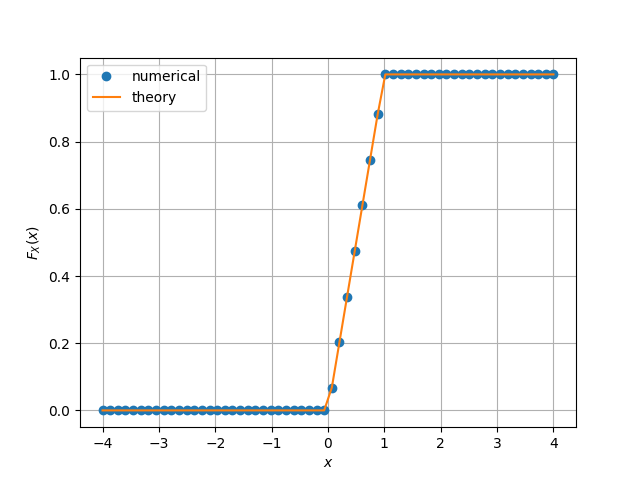
\includegraphics[width=\columnwidth]{./figs/uni_cdf.png}
\caption{The CDF of $U$}
\label{fig:uni_cdf}
\end{figure}

%
\item
Find a theoretical expression for $F_{U}(x)$.

\solution
The CDF of $U$ is given by
		\begin{align}
			F_U(x) = \pr{U \leq x} = \int_{-\infty}^{x}p_U(u)du
		\end{align}
There are three cases:
		\begin{enumerate}
			\item $x < 0$ : \\ $p_X(x) = 0$, and hence $F_U(x) = 0$.\\
			\item $0 \leq x \leq 1$ : \\ 
				\begin{equation}
					F_U(x) = \int_{0}^{x}du = x
				\end{equation}
			\item $x > 1$: \\ \[F_U(x) = \int_{0}^{1}du = 1\]
		\end{enumerate}
Therefore,
		\begin{align}
			F_U(x) = 
			\begin{cases}
				0 & x < 0 \\
				x & 0 \leq x \leq 1 \\
				1 & x > 1
			\end{cases}
		\end{align}\\
\item
The mean of $U$ is defined as
%
\begin{equation}
E\sbrak{U} = \frac{1}{N}\sum_{i=1}^{N}U_i
\end{equation}
%
and its variance as
%
\begin{equation}
\text{var}\sbrak{U} = E\sbrak{U- E\sbrak{U}}^2 
\end{equation}

Write a C program to  find the mean and variance of $U$.\\

\solution
The C program can be found here
\begin{lstlisting}
codes/uni_mean_var.c
\end{lstlisting}

The computed mean is 0.500137 and the variance is 0.083251.\\

\item Verify your result theoretically given that
\end{enumerate}
%
\begin{equation}
E\sbrak{U^k} = \int_{-\infty}^{\infty}x^kdF_{U}(x)
\end{equation}
\solution
\begin{align}
	E\sbrak{U} &= \int_{-\infty}^{\infty}xdF_U(x) \\
	&= \int_{-\infty}^{\infty}xp_U(x)dx \\
	&= \int_{0}^{1}xdx = \frac{1}{2}
\end{align}
This verifies the empirical mean of 0.500137\\

\begin{align}
	E\sbrak{U^2} &= \int_{-\infty}^{\infty}x^2dF_U(x) \\
	&= \int_{-\infty}^{\infty}x^2p_U(x)dx \\
	&= \int_{0}^{1}x^2dx = \frac{1}{3}
\end{align}


\begin{align}
	\text{var}\sbrak{U} &= E\sbrak{U^2} - \left(E\sbrak{U}\right)^2 \\
	&= \frac{1}{3} - \frac{1}{4} = \frac{1}{12} 
\end{align}
This verifies the empirical variance of 0.083251\\
\section{Central Limit Theorem}
%
\begin{enumerate}[label=\thesection.\arabic*
,ref=\thesection.\theenumi]

%
\item
Generate $10^6$ samples of the random variable
%
\begin{equation}
X = \sum_{i=1}^{12}U_i -6
\end{equation}
%
using a C program, where $U_i, i = 1,2,\dots, 12$ are  a set of independent uniform random variables between 0 and 1
and save in a file called gau.dat\\

\solution
The required samples are  generated by the C file in Question 1.1\\
%
\item
Load gau.dat in python and plot the empirical CDF of $X$ using the samples in gau.dat. What properties does a CDF have?

\solution The CDF of $X$ is plotted in Fig. \ref{fig:gau_cdf}
\begin{figure}[h!]
\centering
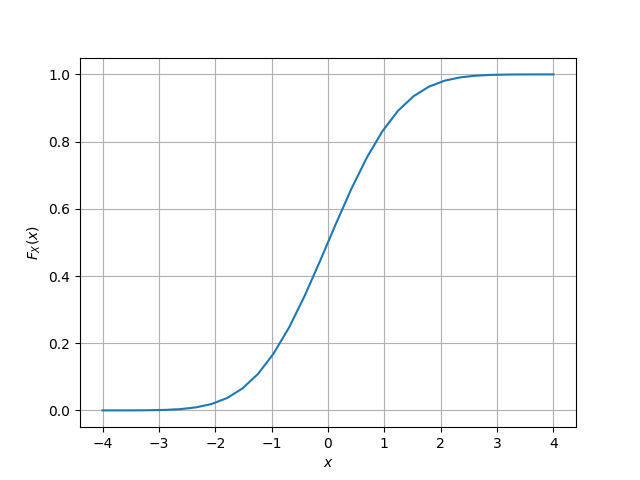
\includegraphics[width=\columnwidth]{./figs/gau_cdf.png}
\caption{The CDF of $X$}
\label{fig:gau_cdf}
\end{figure}\\

The code can be found at
\begin{lstlisting}
codes/gau_cdf_plot.py
\end{lstlisting}
The properties of CDF of $X$ are:
		\begin{enumerate}
			\item The CDF is monotonically increasing
			\item $\lim\limits_{x \to -\infty}F_X(x) = 0$
			\item $\lim\limits_{x \to \infty}F_X(x) = 1$\\
		\end{enumerate}
\item
Load gau.dat in python and plot the empirical PDF of $X$ using the samples in gau.dat. The PDF of $X$ is defined as
\begin{align}
p_{X}(x) = \frac{d}{dx}F_{X}(x)
\end{align}
What properties does the PDF have?

\solution The PDF of $X$ is plotted in Fig. \ref{fig:gau_pdf} using the code from
\begin{lstlisting}
codes/pdf_gau_plot.py
\end{lstlisting}

The properties of pdf of $X$ are:
		\begin{enumerate}
			\item $p_X(x) = p_X(-x)$
			\item $\int_{-\infty}^{\infty}p_X(x)dx = 1$
		\end{enumerate}
	
\begin{figure}[h!]
\centering
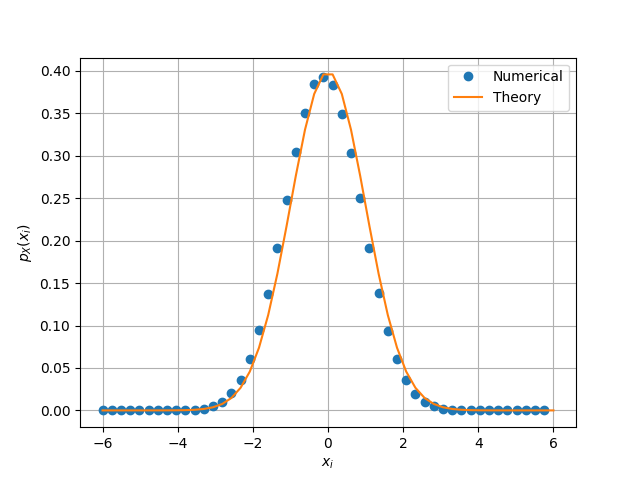
\includegraphics[width=\columnwidth]{./figs/gau_pdf.png}
\caption{The PDF of $X$}
\label{fig:gau_pdf}
\end{figure}

\item Find the mean and variance of $X$ by writing a C program.

\solution
The code can be found at 
\begin{lstlisting}
codes/gau_mean_var.c
\end{lstlisting}

The computed mean is -0.000417 and the computed variance is 0.999902.\\

\item Given that 
\begin{align}
p_{X}(x) = \frac{1}{\sqrt{2\pi}}\exp\brak{-\frac{x^2}{2}}, -\infty < x < \infty,
\end{align}
repeat the above exercise theoretically.

\solution
The mean is given by
		\begin{align}
			E\sbrak{X} =& \int_{-\infty}^{\infty}x\frac{1}{\sqrt{2\pi}}\exp{\brak{-\frac{x^2}{2}}}dx\\
			=& \,\,0\,\,\text{(Since the integrand is odd)}
		\end{align}

		\begin{align}
			\text{var}\sbrak{X} &= E\sbrak{X^2} - \left(E\sbrak{X}\right)^2 \\
			&=\int_{-\infty}^{\infty}x^2\frac{1}{\sqrt{2\pi}}\exp{\left(-\frac{x^2}{2}\right)}dx\\
			\begin{split}
			 &= x\int_{-\infty}^{\infty}x\frac{1}{\sqrt{2\pi}}\exp{\left(-\frac{x^2}{2}\right)}dx \\&\hspace{3em} -\int_{-\infty}^{\infty}\int x\frac{1}{\sqrt{2\pi}} \exp{\left(-\frac{x^2}{2}\right)}dx
			\end{split}\\
			&= \left.-xe^{-\frac{x^2}{2}}\right|_{-\infty}^{\infty} + \int_{-\infty}^{\infty} e^{-\frac{x^2}{2}}\\
		\end{align}
Substituting limits we get $E[x^2] = 1$


\end{enumerate}
\section{From Uniform to Other}
\begin{enumerate}[label=\thesection.\arabic*
,ref=\thesection.\theenumi]
%
\item
Generate samples of 
%
\begin{equation}
V = -2\ln\brak{1-U}
\end{equation}
%
and plot its CDF. 

\solution
The codes can be found at
\begin{lstlisting}
codes/v_samp.c
codes/cdf_v_plot.py
\end{lstlisting}
and the CDF is plotted in Figure \ref{fig:v_cdf}.

\begin{figure}[h!]
\centering
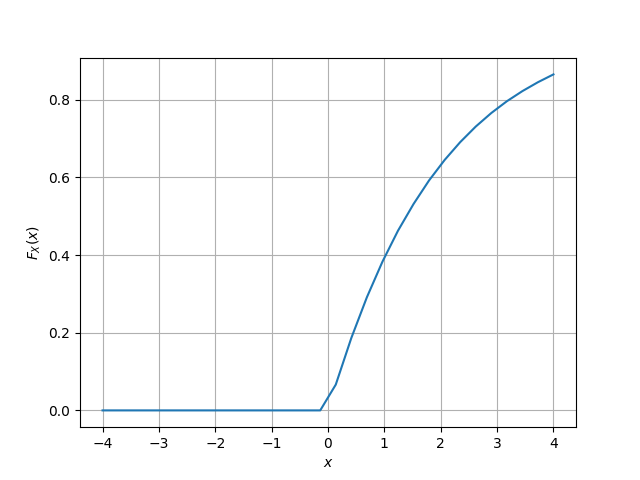
\includegraphics[width=\columnwidth]{./figs/v_cdf.png}
\caption{The CDF of $V$}
\label{fig:v_cdf}
\end{figure}

\item Find a theoretical expression for $F_V(x)$.

\solution
The function 
		\begin{equation}
			V = f(U) = -2\ln{(1 - U)}
		\end{equation}
is monotonically increasing in [0, 1] . Hence, it is invertible and the inverse function is given by
		\begin{equation}
			U = f^{-1}(V) = 1 - \exp{\left(-\frac{V}{2}\right)}
		\end{equation}
	
		\begin{align}
			F_V(x) &= \pr{V < x}\\
			&= \pr{f(U) < x}\\
			&= \pr{U < f^{-1}(x)}\\
			&= \pr{U < 1 - \exp{\left(-\frac{x}{2}\right)}}\\
			&= F_U\left(1 - \exp{\left(-\frac{x}{2}\right)}\right) \\
			\implies F_V(x) &= 
			\begin{cases}
				0 & x < 0 \\
				1 - \exp{\left(-\frac{x}{2}\right)} & x \geq 0
			\end{cases}
		\end{align}

\end{enumerate}

\end{document}
